\documentclass[12pt, letterpaper]{article}
\usepackage{amsmath}
\usepackage{hyperref}
\usepackage{listings}
\usepackage{caption}
\usepackage{subcaption}
\usepackage[letterpaper]{geometry}
\usepackage[doublespacing]{setspace}
\usepackage{titling}
\usepackage{graphicx}

\setlength{\droptitle}{-4cm}

\begin{singlespace}
\title{Parallelize Serial Graph Analytics With Data Centric Graph Primitives}
\author{Chenshan Yuan}
\date{}

\begin{document}
\maketitle

\subsection*{Introduction}
A lot of big data problem can be interpreted as graph problems. For large-scale graphs, the performance of the analytic tools is important. Gunrock is the state-of-art graph analytics library on GPU.\cite{DBLP:journals/corr/WangPDWYWOYLRO17} The goal of this project is to explore Gunrock library programmability and and provide users an alternative high level interface in Python. NetworkX is a popular graph analytic library programmed in Python. \cite{hagberg-2008-exploring} NetworkX provides  a lot of  graph primitives  that  are implemented ideal for CPU. The challenge is to parallelize serial graph algorithms in Gunrock framework.  


\subsection*{Background}

Gunrock has a data-centric framework. A subset of edges or vertices in a graph is represented as a frontier. Gunrock provides a frontier operator abstraction. Each graph analytic algorithm then can be interpreted as a iterative process of operation executed on a frontier. Given this data-centric framework, it's possible to translate or map serial and iterative graph algorithms into a parallel graph algorithms suited for GPU.  

\subsection*{Approach}

In Gunrock framework, there are three traversal operators: advance, filter and segmented intersection.  There is also a  computer operator that can be fused with  one of the traversal operators.  Each  operator has a different functionality. An advance operator  generates a new frontier from current frontier by visiting  neighbors of  current frontier. A  filter operator generates a new frontier  by choosing a subset  from current frontier given programmer-specified  condition.  A compute operator defines an operations to be done  on all elements  in the input frontier. A segmented intersection takes two frontier and return number of intersections  and  intersected node IDS as new frontier.

Given Gunrock's operator level abstraction, it's  critical to characterize a  serial graph algorithm and  map it to Gunrock operators. Shown in Figure 1 is a  Bellman For d algorithm for solving SSSP problem in a graph. This piece of algorithm has been broken down into sections of code which each section represents an operator in Gunrock framework. Shown in  Figure 2 is Bellman Ford algorithm  interpreted in Gunrock framework.

%begin figure is a  floating environment
\begin{center}
\captionsetup{type=figure}
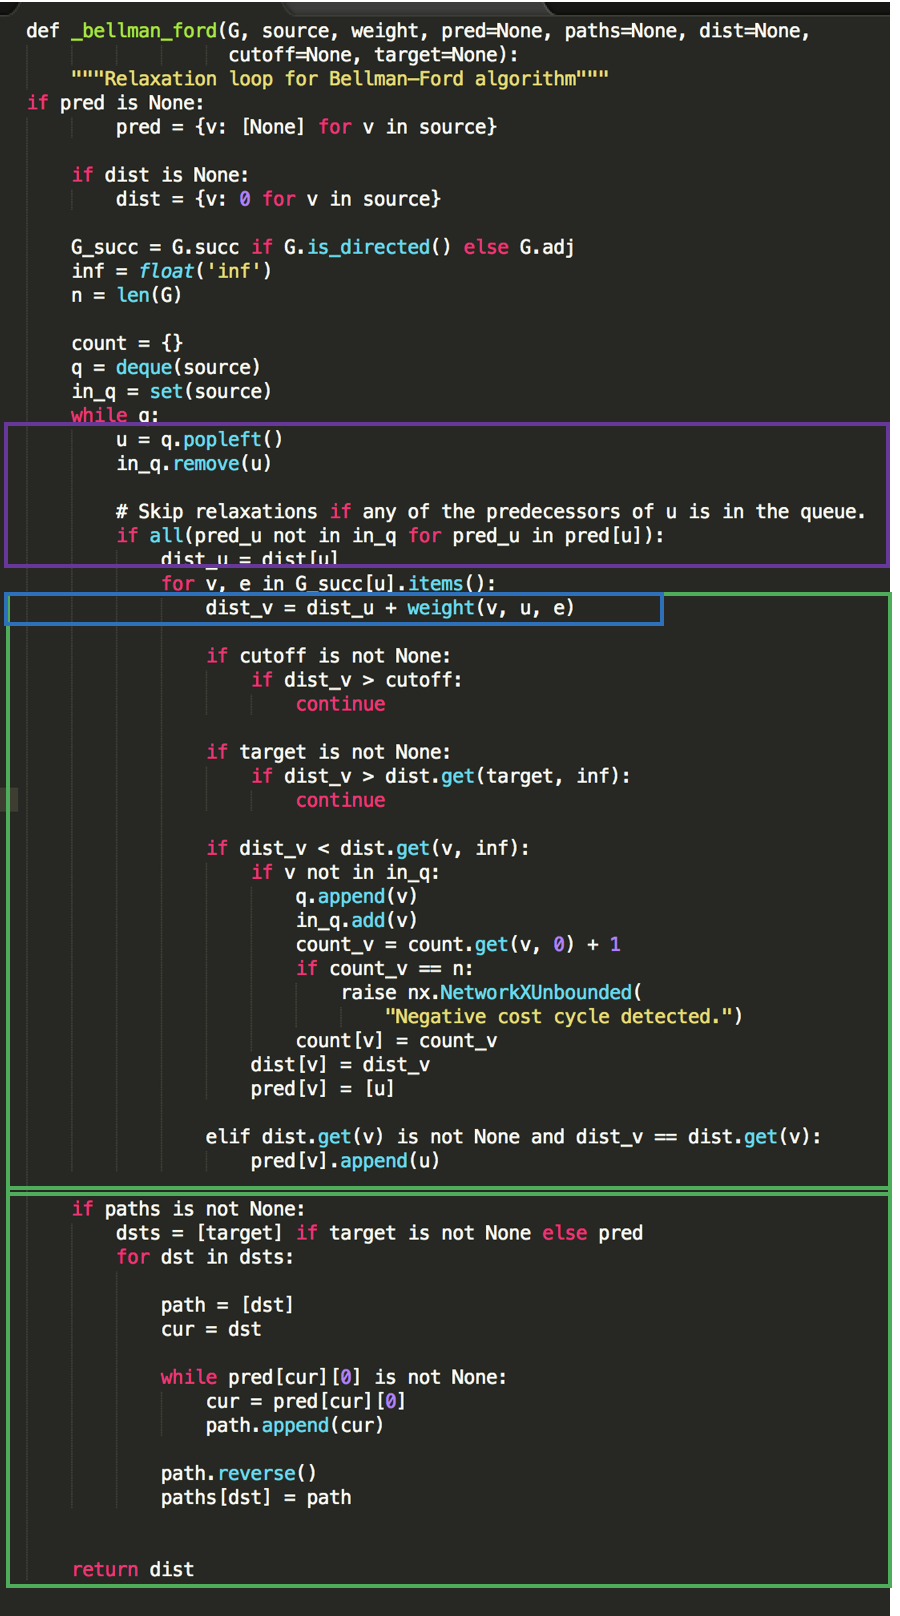
\includegraphics[width=.5\linewidth]{sssp.png}
\captionof{figure}{SSSP, Bellman Ford.}
\end{center}

\begin{center}
\captionsetup{type=figure}
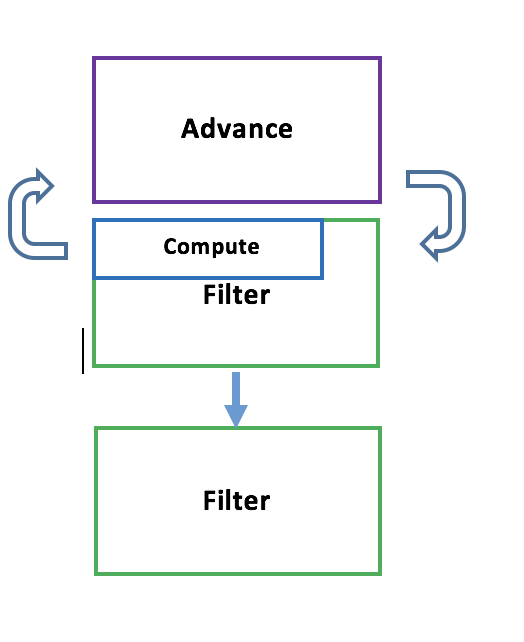
\includegraphics[width=.5\linewidth]{gunrocksssp.png}
\captionof{figure}{SSSP, Bellman Ford in Gunrock framework.}
\end{center}


\bibliographystyle{abbrv}
\
\bibliography{ref}  

\end{singlespace}
\end{document}

